\section{Material and Methods}

\subsection{The objective} 

This study aims to demonstrate the effectiveness of Reinforcement Learning algorithms in optimizing parameters for network-scale brain simulation. Furthermore, it is a mean to test Potjans and Diesmann's thesis, sustaining that the connectivity of a biological network is the main factor that contributes in the shaping of firing rates.
It could be seen as an extension to Potjans and Diesmann's research, attempting to leave the task of finding the right parameters to an algorithm, in a sense reverse engineering the recorded activity rather than reaching it through induction. 


\subsection{The methodology} 

A modified version of the DDPG algorithm was trained on a simulation of a brain column, where it was able to modify different parameters in different settings, explained in detail later. Its objective was to minimize the difference between the firing rates of the simulation and the ones recorded from in vivo settings. Specifically, the activity it was trying to match was the one provided from the study of De Kock et al. \cite{kock}, that has also been used from Potjans and Diesmann to compare their result. This way a comparison between the three results will be coherent.

The data \cite{kock} comes from rats in resting state, with the head fixed in position, and has been chosen over other recordings because it has been found to be the more complete and reliable, even if it only includes the activity of excitatory populations. 


This experiment provides both an instrument for future research to exploit breakthroughs in close fields, like machine learning, and the opportunity to understand which how changing parameters shapes the output of a network.

In order to achieve that understanding, the experiment was repeated 4 times, each of which has different parameters modified:
\begin{enumerate}[noitemsep]
	\item Neuron parameters
	\item Synapses parameters
	\item Connection probabilities 
	\item All at once
\end{enumerate}
Refer to appendix \ref{appendix_a} for a more accurate description of what was changed in each setting.


\subsection{The environment}

\myparagraph{The brain column} 
The environment in which the agent acted was a scaled version of the Potjans and Diesmann column, where the number of neurons is $8 \cdot 10^3$ instead of $8 \cdot 10^4$. That was necessary to reduce computational time. The neurons belong to excitatory and inhibitory populations, and are organized on four different layers, that represent the layers 2/3, 4, 5 and 6 in the sensory cortex of a rat.

For the simulated column to be a suitable environment for training a DDPG agent, it needs to provide both feedback on its activity and a way to change it.

\myparagraph{The reward}
The only input to the agent was the reward, calculated as the negative squared root of the absolute difference between the firing rates of the excitatory neurons in the layers 2/3, 4, 5 and 6 recorded from the somatosensory cortex of a rat \cite{kock}, and the firing rates of the excitatory neurons in the same layers. Computing the reward in this way is not optimal, because the agent doesn't know in which layer the error was, but right now it doesn't seem to exist a better method.  

\myparagraph{The parameters} 
All the starting parameters are the ones provided by Potjans and Diesmann, in particular the ones regarding synapses and connections, while neuron parameters are also the same of the random balanced network. The agent directly changes them, as will be described later. Parameters aren't constrained in any way, other than trying to reduce their change and not adding connections between populations that were not already linked, for example when connection probability equals 0.

\myparagraph{Potjans and Diesmann's Model} 
The starting point of this study is the model developed by Potjans and Diesmann \cite{potjans}, as it was for many others \cite{wagatsuma2011layer}, \cite{linden2011modeling}, \cite{shimoura2018reimplementation}. 

The authors \cite{potjans} expanded the random balanced network \cite{brunel} to a multi-layered case, comprising integrate-and-fire neurons, exponential currents and following the parameterization of the starting model. In particular, to achieve biologically plausible behaviors of the network, the synaptic relative strength of inhibitory connections is multiplied by a factor of 4.

The model of cortical column considered is still assumed to be anatomically uniform, with only 2 populations of neuron, distributed in different proportion between 4 layers. In reality there are many different kind of neurons and other cells, but trying to simulate those is both very computationally expensive and not that determinant in terms of the considered outcome.

Their simulation aims to be the minimal extension of the mono-layered model of the random balanced network. It only integrates static connections between neurons, and the set of cell types is the smallest typically distinguished in experiments.

The focus of this research was over the role of connectivity between populations of neurons in shaping firing rates. To achieve a proper connectivity map to emulate the activity of biological network, the authors \cite{potjans} combined data from previous physiological and anatomical studies on mammal's neocortex, through an algorithmic procedure and following constraints to adhere with biological data. 

The connectivity maps belonged to different mammals and different areas, because the coherent data from the same area and animal was not available. Furthermore, anatomical and physiological recordings produce different biases, that was taken into account in the study.
Nevertheless, the connection probabilities originate from this data will only be applicable over a theoretical generic column, not a specific one. 

The parameters were chosen in a way such that excitatory postsynaptic potentials has an average amplitude of 0.15 mV with a rise time of 1.6 ms, imitating the in vivo situation. The delays in the network are independent of the layer, with delays of excitatory populations on average twice as long as delays of inhibitory populations, based on in vivo data \cite{thomson2003interlaminar}. Excitatory connections from layer 4 to layer 2/3 are doubled, because the data was on them was inconclusive, but they affect only marginally ongoing activity.

The firing rates were compared with the values recorded on other studies \cite{kock} and the trend showed in both cases was similar, so that the lowest rates were shown in layers 2/3 and 6, and the highest in layer 5 (Figure \ref{fig:potjans_barplot}), yet it wasn't accurately matched. 

\begin{figure}[h]
	\raggedleft
	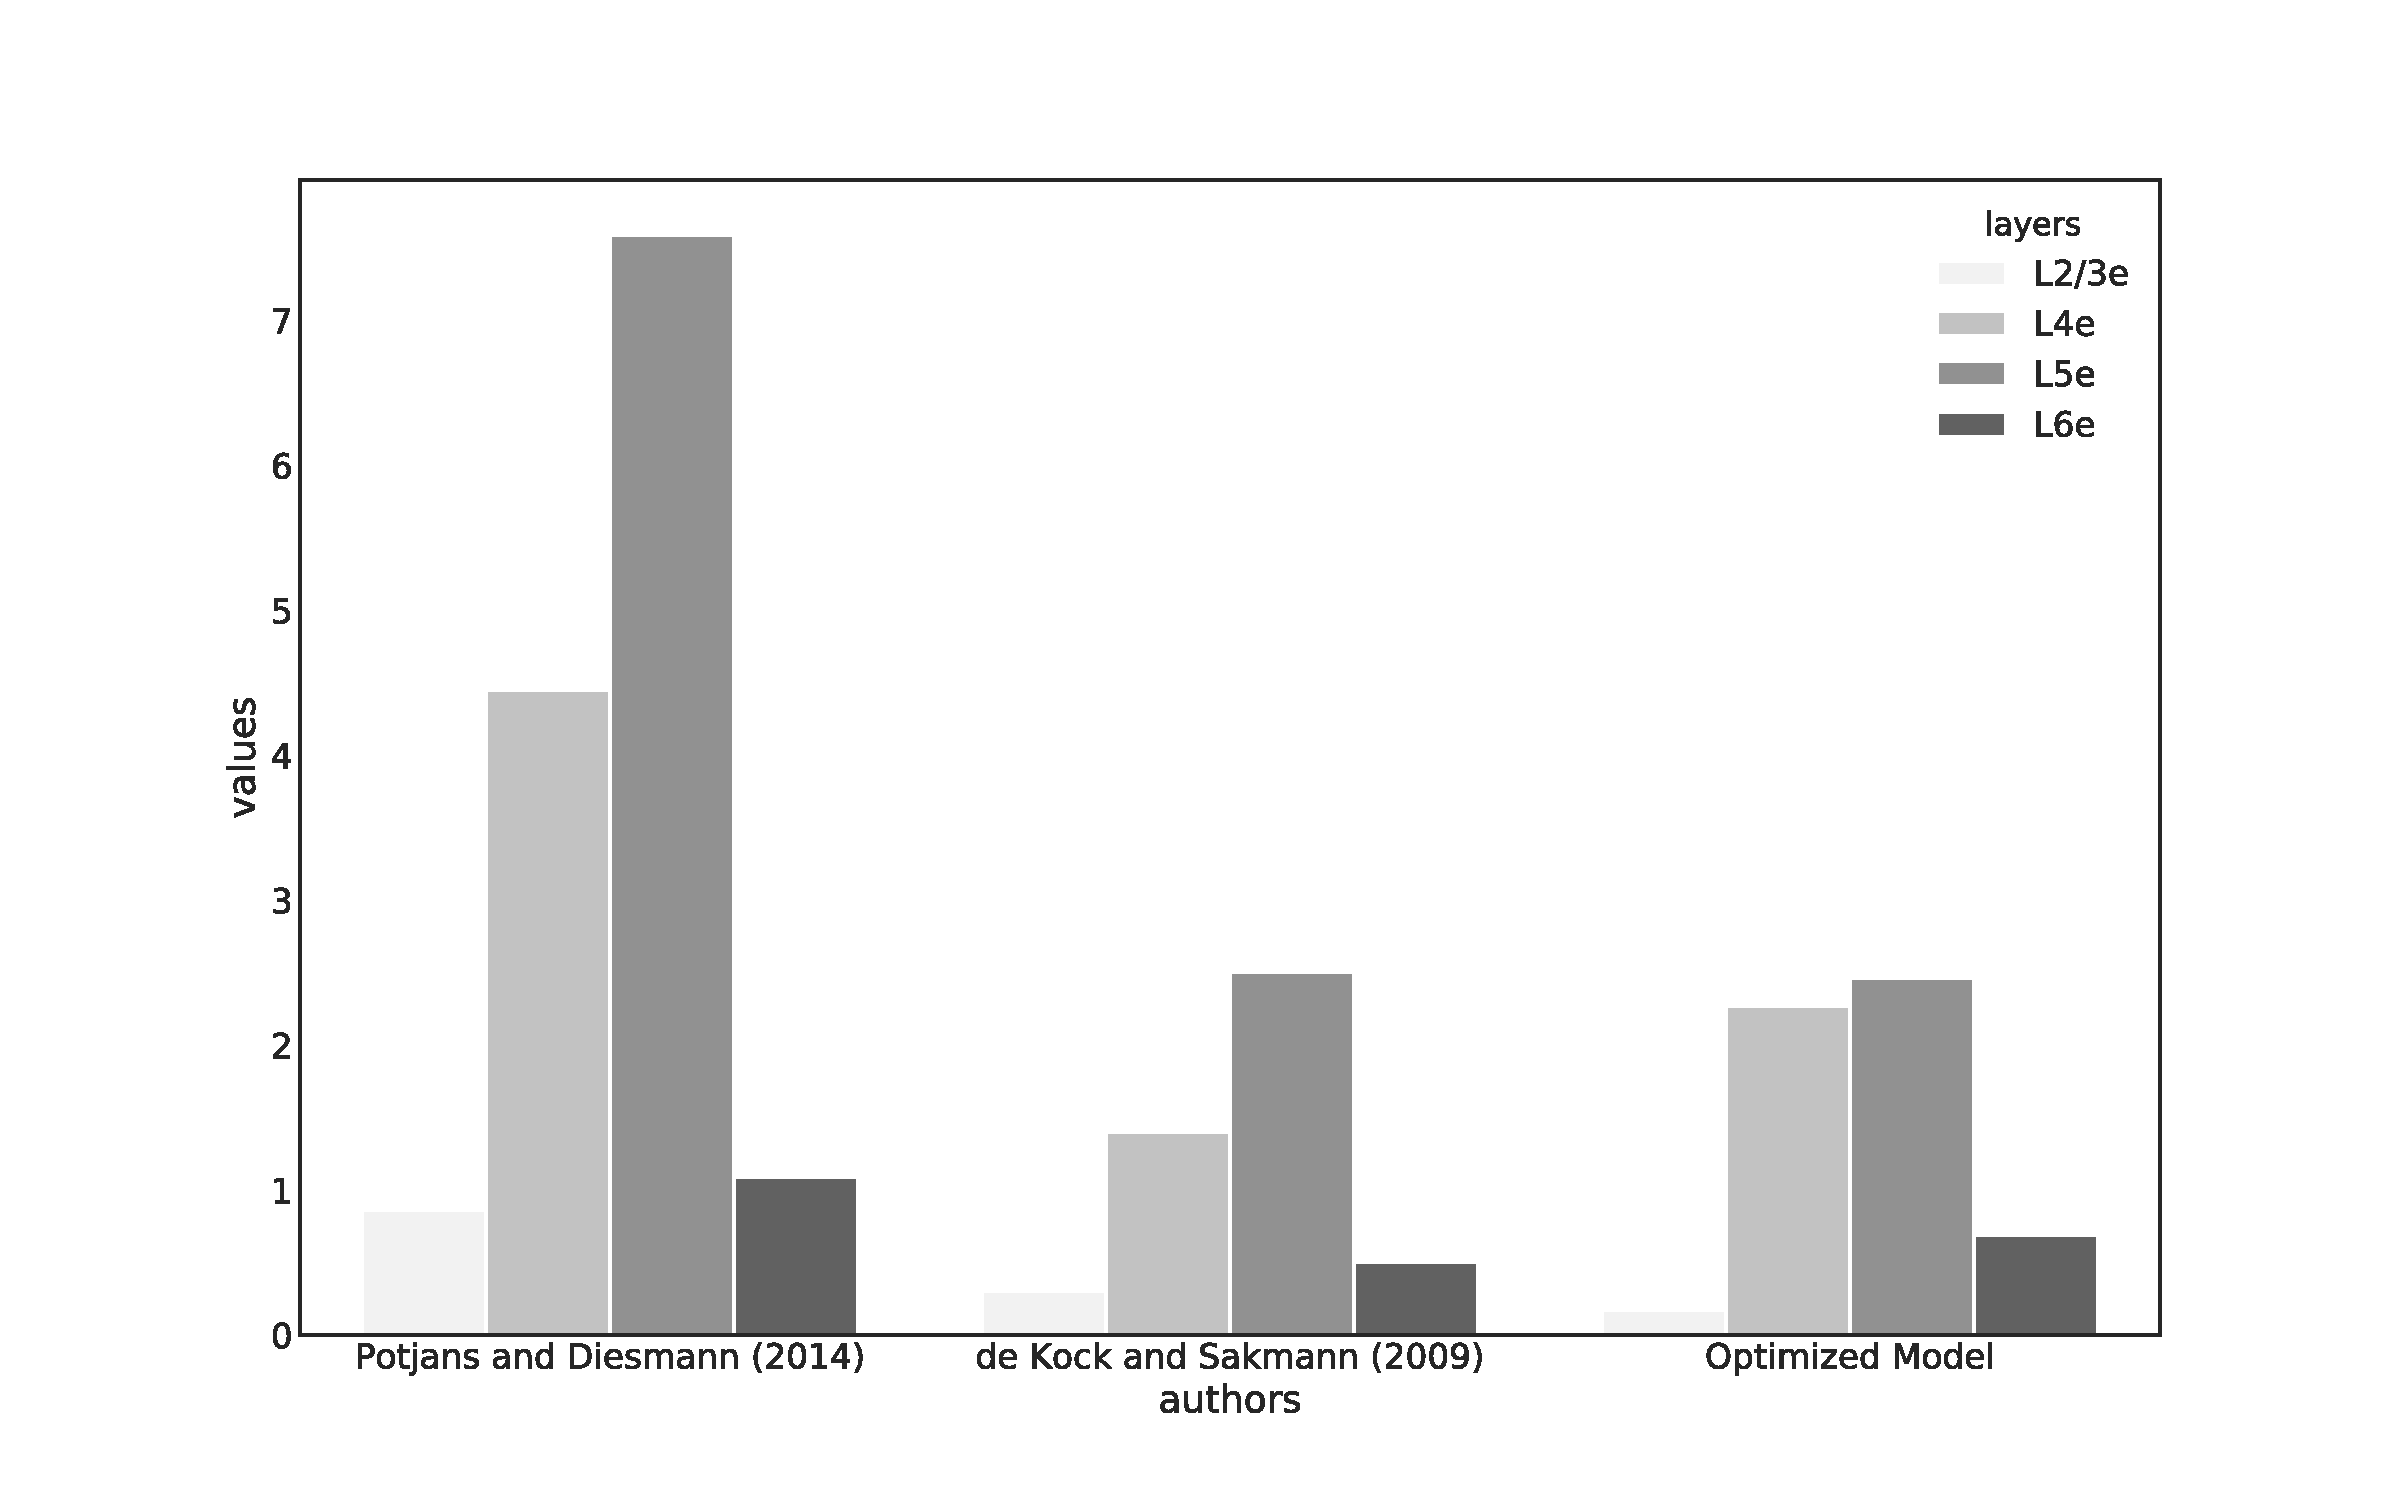
\includegraphics[scale=0.40]{pictures/potjans_barplot.pdf}
	\caption{Comparison of firing rates from the different studies}
	\label{fig:potjans_barplot}
\end{figure}

\subsection{The agent}

\myparagraph{The algorithm} 
As already said, the model deployed in this study is a modified version of DDPG. The choice of the algorithm was based on many factors, but the most important feature was that it had to be able to change the parameters of the simulation, that are continuous values, so it had to be able to compute continues actions. This is best achieved by algorithms that are intended to be used in the robotic context, exactly like DDPG. 

\myparagraph{Adaptation to the bandit problem} 
Being the environment shaped as a multi-armed bandit problem, the agent find itself always in the terminal state, so it doesn't have to compute state Q-values for concatenated observations, and the DDPG model could be simplified, removing the target networks.

\myparagraph{Parameters update}
The output layer of the actor model has a hyperbolic tangent as activation function, that bounds the output values between 0 and 1. This leaves the possibility to modulate the effect that each action has on the parameters. Specifically, if the $p$ is the vector of parameters to change, the actions are the vector $a$ of values $a_1, a_2 \ldots a_n$ between 0 and 1 with $n$ as the number of parameters to change, and $k > 1$ a constant that constrains the action, the update was done by the equation:
\begin{equation}
	p^{new}_i = p_i + \frac{a_i \cdot p_i}{k}
\end{equation}
That is important to reduce the space where the agent looks for the values of the parameters, but has to be manually tuned. 


\subsection{The whole model}
Having described how the main parts of the model work, here it is an overview of the whole training process.

\myparagraph{Generating the agent} 
Following the original paper \cite{lillicrap} the agent is created with the weights of both the actor and the critic initialized in such a way so that the first actions that it takes are close to zero, that helps a stable and reproducible training: in fact it could happen that a particular set of starting weights produce actions such that the model is already close to the solution, but that would be just random. 

\myparagraph{The noise}
Then each of the first actions of the agent will be just the noise generated by a Gaussian distribution with 0 as mean and standard deviation equal to 1. The noise is maximum in the start so that the agent is forced to explore a relatively large space before deciding were to focus. After around 7000 iterations the noise will be halved (its half-life is $7\cdot10^4$).

\myparagraph{The interaction with the environment}
When the agent takes an action what it really happens is that: 
\begin{enumerate}[noitemsep]
	\item The actor generates a vector of actions
	\item The agent adds the noise to the vector
	\item The vector get fed in the environment and divided by $k$
	\item The vector is turned into a sort of dictionary, where every value is associated with its key
	\item The brain column is built retrieving the values using the keys
	\item The brain column is simulated for 1000 ms, and the spikes of 500 ms are counted and averaged with respect to their population and layer
	\item The resulting fire rates are returned to the program
\end{enumerate}

\myparagraph{Training the agent} 
The agent is trained on a random batch of past episodes, using the recorded data. The randomness helps with stabilizing the training, and training on a batch is much more efficient for neural networks on GPU architectures, thank to parallelization.

Usually, after the first few thousands of training steps, the model converges to low values of errors, and slowly approaches the 0 error. This deceleration could be due to the problem mentioned above of optimizing multiple target values at the same time. The noise is critical in this period, because without it the agent would just repeat the action he experienced to yield the best results, and the learning process would stop.
